\begin{figure}[ht]
    \centering
    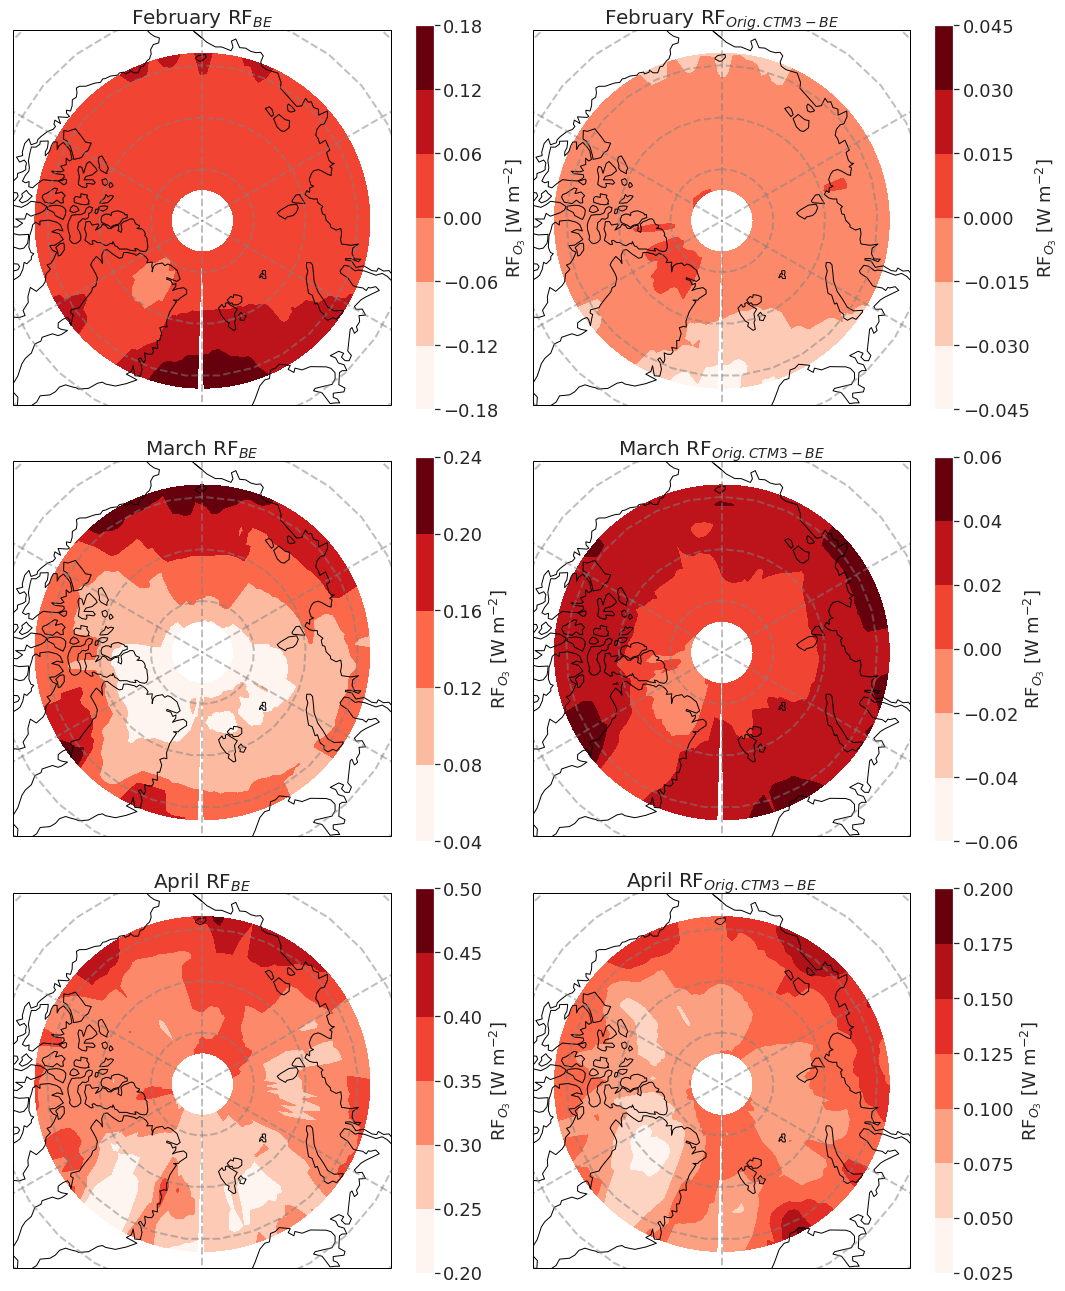
\includegraphics[width = \linewidth]{Chapter6_Results/images/RF/RF_USE/BEOrig_RF_polar_FebApr_2013.png}
    \caption{Polar RF-field (in Wm$^{-2}$) in 2013 for the total tropospheric column up to the tropopause, produced using the BE-branch (left columns) and the Orig. CTM3 RF minus the BE-branch RF (right columns) for the months February (top figures), March (middle figures) and April (bottom figures)}
    \label{fig:BEorig_RF_polar_FebApr_2013}
\end{figure}